\documentclass[a4paper,12pt,russian]{article}

\usepackage{geometry}
\geometry{a4paper,top=2cm,bottom=2cm,left=4cm,right=2cm} %% отступы и т.п.
%\linespread{1.3}

%% чтоб работал русский язык
\usepackage[utf8]{inputenc}
\usepackage[russian]{babel}

%% для математических символов
\usepackage{amsmath, amsthm, amssymb}

%% листинги кода
\usepackage{listings}
%:\usepackage{courier}
\lstset{
  language=c++,
  basicstyle=\footnotesize\ttfamily,
  commentstyle=\footnotesize\sffamily\emph,
  keywordstyle=\bfseries,
  stringstyle=\ttfamily,
  numberstyle=\tiny,
  numbers=left,
  captionpos=b,
  floatplacement=h
}

%% картинки
\usepackage[pdftex]{graphicx}
\usepackage[small, bf, labelsep=period]{caption}
\graphicspath{{img/}}
\usepackage{multicol}

%% листинги программ
\usepackage{moreverb}
\usepackage[noend]{algorithmic}
\algsetup{indent=2em, linenosize=\small, linenodelimiter=}

%% чтоб первый абзац был с отступом
\usepackage{indentfirst}

%% всякое для удобства разметки
%\newcommand{\remark}[1]{~~\textit{\textbf{(#1)}}}
\newcommand{\remark}[1]{\footnote{#1}}

\newcommand{\picref}[1]{\textbf{рис.~\ref{#1}}}

\newcommand{\code}[1]{\textsf{#1}}

\newtheorem*{definition}{Определение}

\begin{document}
\begin{titlepage}
	\begin{center}
		\Large
		Московский~государственный~университет\\
		имени М.В.~Ломоносова\\[0.5em]
		\large
		Факультет~вычислительной~математики~и~кибернетики\\
		Кафедра~системного~программирования
	\end{center}

\vskip 14em
	\begin{center}
		\LARGE
		Дипломная работа\\
		\textbf{``Восстановление определений классов на языке Си++ посредством динамического анализа бинарного кода''}\\
	\end{center}
\vskip 6em
	\begin{flushright}
		\large
		Выполнил~студент 527~группы\\
		Прохоренков~П.В.\\
		\vspace{2cm}
		Научный руководитель\\
		к.ф-м.н, доц. Чернов~А.В.\\
\end{flushright}
\vfill
	\begin{center}
		\Large
		Москва\\
		2010
	\end{center}
\end{titlepage}

\tableofcontents

\newpage

\addcontentsline{toc}{section}{Введение}
\section*{Введение}
\emph{Обратная инженерия} является процессом анализа системы, имеющим 2 цели: восстановление компонент системы и их взаимных связей, и создание описания системы в другой форме с более высоким уровнем абстракции

\emph{Декомпиляция} представляет собой составную часть процесса обратной инженерии, это трансформация программы, которая восстанавливает код на языке высокого уровня по исполняемому файлу программы, ассемблерному коду, либо по любому представлению низкого уровня.
Декомпиляция является обратным преобразованием к компиляции.

Декомпиляция может использоваться для
\begin{itemize}
\item{\textbf{Поиска ошибок, уязвимостей, вредоносного кода}} Например, в более не поддерживаемом программном обеспечении, поставляемом в без исходных кодов.
\item{\textbf{Верификации}} С помощью декомпиляции задачу верификации двоичного кода можно свести к задаче верификации кода на языке высокого уровня.
\item{\textbf{Восстановления алгоритмов работы}}
\item{\textbf{Обеспечения совместимости программ}} Например, создание модулей расширения для программ, к которым не существует доступных описаний двоичных интерфейсов.
\item{\textbf{Оптимизации}} Например, старая программа, скомпилированная для старого процессора, может быть перекомпилирована под новый с использованием всех существующих оптимизаций.
\item{\textbf{Переноса на другую платформу}} После декомпиляции кода, можно скомпилировать его для другой платформы, для которой существует компилятор выходного языка декомпилятора.
\item{\textbf{Восстановления утраченного исходного кода}}
\item{\textbf{Восстановления протоколов обмена программ, исходные коды которых утрачены}}
\end{itemize}

В данной работе будет рассматриваться декомпиляция программ, изначально написанных на языке Си++.
Язык Си++ является универсальным языком с поддержкой объектно-ориентированной парадигмы программирования \cite{strstr}. Этот язык получил широкое распространение, и существует множество программ, написанных на нем.

Одной из подзадач декомпиляции является восстановление типов данных высокого уровня, как базовых, так и производных.
В программах на языках высокого уровня разработчику ПО доступно множество различных типов данных.
В их число входят и составные типы данных, во многих случаях размещаемые в динамической памяти.

В ассемблере отсутствует информация о структурах данных, использованных исходной программой.
Все операции доступа к полям данных структур представляются в виде операций с отдельными ячейками памяти с использованием адресной арифметики.
К примеру, в коде на \picref{field_ref_lst}, операция доступа к полю \code{b} структуры \code{S} на платформе \code{x86} может иметь вид, показанный на \picref{field_ref_asm_lst}.

\begin{figure}
\begin{lstlisting}
struct {
  int a;
  int b;
} s;

void f() {
  s.b = 1;
}
\end{lstlisting}
\caption{Пример доступа к полю структуры}
\label{field_ref_lst}
\end{figure}

\begin{figure}
\begin{lstlisting}[language={[x86masm]Assembler}]
movl $s, %eax
movl 1, 4(%eax)
\end{lstlisting}
\caption{Пример ассемблерного кода для доступа к полю структуры}
\label{field_ref_asm_lst}
\end{figure}

Таким образом, утрачивается информация о структурах данных.
Использование статических методов анализа для решения задачи восстановления составных типов осложняется тем, что необходимо проведение анализа потоков данных и управления, точное восстановление которых статическими методами невозможно.

Динамический анализ во многих случаях позволяет получать недостающую информацию. Но к числу его недостатков надо отнести необходимость запуска исследуемой программы.
Это требует получения входных данных, в обработке которых будут задействованы все интересующих исследователя участки кода.
Также, в некоторых случаях необходимы большие вычислительные ресурсы из-за накладных расходов инструментария анализа.

Знание иерархии классов, используемых в анализируемой программе может иметь большое значение для специалиста. Например, многие алгоритмы могут быть распознаны по используемым в них структурам данных.

Данная работа посвящена восстановлению иерархий классов по бинарному коду в программах, написанных на языке Си++.
Восстановление проходит при помощи динамического анализа программы.

\newpage
\section{Постановка задачи}
Требуется разработать и реализовать инструментальное средство, использующее методы динамического анализа для восстановления иерархии классов, используемых в анализируемой программе.
Результатом работы средства должно являться наиболее полно восстановленное:
\begin{enumerate}
\item Множество классов.
\item Частичное отношение наследования между классами.
\item Таблица виртуальных функций для каждого из классов.
\item Список полей для каждого из классов.
\item Частичное отношение ассоциации между классами.
\end{enumerate}

При реализации необходимо использовать инструментальную среду для динамического анализа программ \code{Valgrind}.
Требуется реализовать поддержку языка Си++ для написания инструментов в среде \code{Valgrind}.

\newpage
\section{Методы и средства обратной инженерии классов по бинарному коду}
\label{reverse_eng_overview}
Задаче восстановления иерархий классов уделено недостаточно внимания в литературе.
Существует несколько публикаций, затрагивающих вопрос восстановления иерархий с использованием статического анализа исполняемых файлов.

Работа ``Reversing C++'' \cite{reversing_cpp} описывает методы такого восстановления применительно к коду, сгенерированному компилятором Microsoft Visual C++.
Авторы использовали среду IDA Pro \cite{ida_pro} для получения ассемблерного кода, и реализовали свой инструмент в виде подключаемого модуля для этой среды.
Метод восстановления использовал многие особенности компилятора, такие как передача указателя \code{this} через регистр \code{ecx}, принятую в компиляторе схему декорирования имён функций, расположение в памяти объектов полиморфных классов.
Описанный метод позволяет восстанавливать полную иерархию классов, если в исполняемом файле присутствует \emph{информация о типах времени выполнения} (\emph{Run-time type info, RTTI}).
Такая информация содержит все данные о наследовании классов и их именах, поэтому правильный разбор структур данных позволяет восстанавливать иерархии классов с большой точностью.
Более сложный случай, который рассмотрен в статье, это случай, когда такая информация отсутствует в исполняемом файле.
В таком случае, восстановление использует данные о таблицах виртуальных функций и конструкторах классов.
В конструкторе унаследованного класса должны быть вызваны конструкторы родительских классов.
Эта информация позволяет восстанавливать некоторую часть иерархии.


Работа ``Using a decompiler for real-world source recovery`` \cite{real_decomp} описывает применение существующих инструментов для декомпиляции программ.
Авторы работы описывают опыт, полученный при декомпиляции реального приложения.
В качестве инструментальный средств были использованы дизассемблер IDA Pro \cite{ida_pro} и декомпилятор Boomerang \cite{boomerang}.
Также, многие участки декомпилированного кода требовали редактирования вручную для улучшения читабельности, либо для приведения кода в компилируемый вид.
Полная иерархия классов была восстановлена на основе информация о типах времени выполнения.
При этом никаких инструментальных средств не было использовано, и разбор всех структур данных и построение иерархии авторы выполнили вручную.

Также, есть работы, посвящённые применению динамического анализа для установления различных свойств программ.

Работа \cite{typechecking} описывает инструмент для динамической проверки программ на языке Си, называемый \code{Hobbes}.
Многие важные программные системы написаны на языке Си.
Язык Си не предоставляет строгих гарантий безопасности типов, и многие типичные ошибки разработчиков ПО не отлавливаются компилятором. Такие ошибки проявляют себя только во время исполнения в виде непредсказуемого поведения программы.
Описываемый инструмент интерпретирует откомпилированную программу, отслеживает информацию о типах во всех участках памяти и регистрах и позволяет находить множество ошибок, связанных с типами данных.

Ошибка доступа к памяти происходит, когда программа производит доступ к неверному участку памяти.
Два примера таких ошибок это чтение из памяти, которая не была выделена и чтение из выделенной, но не проинициализированной памяти.

Ошибка типа возникает, когда операция производится с операндами, чьи типы не совместимы с операцией.
Сложение указателя со значением с плавающей запятой, вызов функции с неверным числом аргументов, разыменование значения типа \code{int}, как указателя --- все это ошибки типов.

Нахождение ошибок такого рода, используя статические методы анализа сильно затруднено тем, что необходимо точно находить множества значений переменных.
На данный момент не существует точных методов решения этой задачи.

Для того, чтобы отследить эти ошибки, инструмент поддерживает теневые значения, содержащие признак выделенности и тип для всех значений, доступных целевой программе, которые обновляются и проверяются во время работы программы.
Например, результат команды \code{mul} --- всегда целое значение, результат \code{lea} --- указатель, тип результат инструкции \code{add} определяется типами её аргументов.
Поддерживается возможность получения изначальной информации о типах с использованием исходного кода анализируемой программы.

Инструментальное средство \code{Hobbes} состоит из двух отдельных частей: интерпретатора кода \code{x86}, который обеспечивает работу целевой программы и инструмент для проверки типов --- модуль, вызываемый интерпретатором, когда происходят зарегистрированные события.
Интерпретатор выполняет функции двоичного редактора, или динамического инструментирующего компилятора, лежащего в основе \code{Valgrind} \cite{valgrind}. Сам \code{Valgrind} не был использован, т.к. на момент начала работы он ещё не был выпущен, и реализация своего интерпретатора была кратчайшим путём к построению работающего прототипа.
Важной целью было предоставить анализируемой программе среду выполнения наиболее близкую к обычной работе.
Для этого интерпретатор кода располагается в одном адресном пространстве с анализируемой программой, занимая редко используемую область адресного пространства.
Интерпретатор предоставляет интерфейс, позволяющий инструменту для проверки типов зарегистрировать интересующие его события, например чтение памяти или выполнение определённой инструкции.
Во время выполнения анализируемой программы интерпретатор вызывает функции обратного вызова, когда наступают зарегистрированные события.
Интерпретатор предоставляет различные дополнительные данные о произошедших событиях: адреса в памяти, записываемые или считываемые значения, задействованные регистры.
Инструмент для проверки типов располагается в другом процессе, что решает многие возможные проблемы, такие как необходимость загрузки двух версий одной библиотеки в один процесс.

Работа \cite{abstracttypes} посвящена динамическому выводу абстрактных типов данных.
Такая информация может быть использована для анализа незнакомых программ и упрощения рефакторинга кода.

Даже в сильно типизированных языках, объявленные типы отражают только часть знания разработчика ПО о возможных значениях переменных.
Например, разработчик ПО может использовать тип \code{int} для представления индексов в массиве, измерений, поступающих от датчиков, текущего времени, дескрипторов файлов, счётчиков, адресов в памяти, и для хранения других не связанных друг с другом величин.
Таким образом, восстановление более точной информации, чем выражено типом данных может быть полезным.
Эта информация также может быть использована для последующего анализа, такого как оптимизация анализируемой программы.

Цель этого анализа состоит в восстановлении информации, которая явно не представлена в программе.
Далее, под абстрактным типом будем понимать уточнение типа данных для переменной: две переменные могут быть операндами одной операции тогда и только тогда, когда они имеют один абстрактный тип.
Значения, взаимодействующие в программе должны иметь один и тот же абстрактный тип (иначе, это будет ошибкой в программе), а значения, которые никогда не взаимодействовали, могут быть не связаны.
Строгое понятие взаимодействия определяется одной из следующих четырёх стратегий.
\begin{itemize}
\item \texttt{Поток данных} --- никакие из бинарных операций не являются взаимодействиями. Отслеживается только поток данных, поэтому две переменные имеют один тип, если они принимали одно и то-же значение.
\item \texttt{Поток данных и сравнения} --- две переменные, являющиеся операндами оператора сравнения (например, \code{<} или \code{==}) считаются взаимодействующими.
\item \texttt{Единицы измерения} --- сложение, вычитание и сравнения считаются взаимодействиями, а другие операции, включая умножение и деление --- нет. В итоге, переменным с одним абстрактным типом можно поставить в соответствие одни единицы измерения.
\item \texttt{Арифметика} --- это режим ``по умолчанию'' для данной реализации.
  \begin{itemize}
    \item Сравнения --- взаимодействия между операндами.
    \item Все арифметические (\code{+}, \code{-}, \code{*}, \code{/}, \code{\%}) и побитовые (\code{\&}, \code{|}, \code{\^}) операции --- взаимодействия между операндами и результатом, так что все три значения получают один абстрактный тип.
    \item Операции сдвига (\code{<}\code{<}, \code{>}\code{>}) --- взаимодействия между сдвигаемым значением и результатом операции.
  \end{itemize}
\end{itemize}

В работе описывается реализация описанного алгоритма для двух платформ: \code{Linux/x86} (\code{DynCompB})и \code{Java} (\code{DynCompJ}).
Для проведения динамического анализа на \code{Linux/x86} используется среда \code{Valgrind}.
\code{DynCompB} использует только инструментацию кода анализируемой программы, не заменяя функции выделения и освобождения памяти.
Инструментальное средство поддерживает указатель на структуру, описывающую абстрактный тип, для всех ячеек памяти и регистров.
Для каждой инструкции, осуществляющей доступ к памяти или регистрам вставляется вызов функции-перехватчика.
Эта функция, основываясь на строгом понятии взаимодействия, объединяет абстрактные типы операндов и/или результата инструкции.
Все константы первоначально имеют уникальные абстрактные типы.
При каждом присваивании константы регистру или значению в памяти, присвоенное значение получает уникальный абстрактный тип.
Значения, являющиеся результатами системных вызовов также получают уникальные абстрактные типы.

После работы программы инструментальное средство выдаёт списки переменных, имеющих один абстрактный тип.

Результаты тестирования показывают, что реализация хорошо масштабируется на большие программы.

\newpage
\section{Средства динамического анализа программ}
\label{valgrind_section}
Для реализации данного инструментального средства требовалась среда, позволяющая проводить динамический анализ программ без наличия исходных кодов.
Предоставление возможности для встраивания функций-перехватчиков и подмены функций семейства \code{malloc-free} для анализируемой программы на специальные функции инструментального средства.
Всем этим требованиям отвечает среда \code{Valgrind}.

\code{Valgrind} представляет собой среду для динамического анализа программ, использующую динамическую рекомпиляцию.
Инструментальное средство, реализованное в с помощью \code{Valgrind}'а можно запустить, добавив \[\mbox{\code{valgrind -{}-tool=<toolname>}}\] перед именем анализируемой программы. Указанное средство запускается, загружает анализируемую программу в адресное пространство своего процесса, и затем рекомпилирует машинный код анализируемой программы небольшими блоками прямо во время исполнения, по мере необходимости.
Ядро дизассемблирует блок кода во внутреннее представление (ВП), которое инструментируется и затем переводится обратно в машинный код.
Никакая часть исходного машинного кода анализируемой программы не запускается в исходном виде. Обрабатываемый корректно код включает в себя обычный исполняемый код, динамически скомпилированные библиотеки, динамически сгенерированный код. Единственный код, который не находится под контролем инструмента --- это системные вызовы, но в \code{Valgrind} существует функциональность для получения их побочные эффектов. Множество осложнений возникает при помещении двух программ, анализируемой программы и инструментального средства, в одно адресное пространство. Им приходится 2разделять многие ресурсы, такие как регистры и память.

Цель процесса запуска в том, чтобы поместить ядро \code{Valgrind}, инструментальное средство и анализируемую программу в один процесс и одно адресное пространство. Каждое инструментальное средство предоставляет собой статически скомпилированный исполняемый файл, содержащий код ядра и инструментального средства. Исполняемый файл настраивается на загрузку по нестандартному адресу, который, как правило, является свободным при запуске программы (на Linux это \code{0x38000000}). Ядро \code{Valgrind} сначала инициализирует некоторые подсистемы, такие как управление адресным пространством и свой распределитель памяти. Затем загружается анализируемая программа (секции \code{text} и \code{data}). Затем настраивается сегмент данных и стек анализируемой программы. Далее ядро вызывает функцию инициализации инструментального средства. В конце инициализируются остальные подсистемы: планировщик потоков, обработчик сигналов и т.д. К этому моменту инструментальное средство и анализируемая программа полностью готовы к работе.

\code{Valgrind} транслирует блоки кода при необходимости. Для трансляции блока \code{Valgrind} выбирает инструкции, пока не выполнится одно из следующих условий: достигнут предел числа инструкций (около 50, в зависимости от архитектуры), встречен условный переход, встречено ветвление с неизвестным назначением, обработано более 3 безусловных переходов по известным адресам.

Используемое внутреннее представление является строго типизированным машинно-независимым языком. Во внутреннем представлении может быть использовано неограниченное число временных переменных, значение каждой из которых может быть присвоено только один раз\footnote{Используется так называемое SSA(Static Single Assignment)-представление \cite{aho_compilers}}. Задачу распределения регистров для временных переменных решает ядро \code{Valgrind} при компиляции временного представления в машинный код.

Существует 8 фаз трансляции. Такое большое число --- следствие подхода, используемого \code{Valgrind}. Все фазы берет на себя ядро, за исключением инструментации, выполняемой инструментальным средством. Фазы отмеченные `*' являются архитектурно-зависимыми.

\paragraph{Фаза 1. Дизассемблирование*: машинный код $\longrightarrow$ дерево ВП.}
Дизассемблер переводит машинный код в не оптимизированное дерево ВП. Каждая инструкция дизассемблируется независимо в один или более операторов.

\paragraph{Фаза 2. Оптимизация 1: дерево ВП $\longrightarrow$ плоское ВП.}
Первая фаза оптимизации делает ВП плоским и делает некоторые оптимизации: продвижение копий и констант, свёртывание констант, удаление мёртвого кода, удаление общих подвыражений, и даже разворачивание простых циклов.

\paragraph{Фаза 3. Инструментация: плоское ВП $\longrightarrow$ плоское ВП.}
Блок кода передаётся инструментальному средству, которое изменяет его в соответствии со своими требованиями. Важно, чтобы ВП было плоским к этому моменту, это делает инструментацию более простой.

\paragraph{Фаза 4. Оптимизация 2: плоское ВП $\longrightarrow$ плоское ВП.}
Второй, более простой проход оптимизации выполняет свёртывание констант и удаление мёртвого кода. Эта оптимизация делает жизнь проще для инструментального средства, давая гарантию, что код в последствие будет улучшен.

\paragraph{Фаза 5. Построение дерева: плоское ВП $\longrightarrow$ дерево ВП.}
Построитель дерева переводит плоское ВП обратно в дерево ВП, готовясь к выбору инструкций. Выражения, присвоенные временным переменным, используемым только один раз перемещаются в точку использования этой временной переменной, а присваивание удаляется. Получаемый код может производить чтения из памяти в другом порядке, но запись в память всегда будет идти после чтения.

\paragraph{Фаза 6. Выбор инструкций*: дерево ВП $\longrightarrow$ список инструкций.}
В этой фазе дерево ВП переводится в список инструкций, использующих виртуальные регистры (за исключением тех, которые жёстко привязаны к определённым регистрам). Используется просто жадный алгоритм сопоставления образцов, действующий сверху вниз.

\paragraph{Фаза 7. Распределение регистров: список инструкций $\longrightarrow$ список инструкций.}
Распределитель регистров, использующий линейное сканирование заменяет виртуальные регистры на машинные регистры, вставляя код для сохранения и загрузки значений регистров в память.
Хотя инструкции и зависят от платформы, распределитель регистров является платформо-независимым.
Он использует функции обратного вызова для получения списков регистров читаемых и записываемых данной инструкцией.

\paragraph{Фаза 8. Ассемблер*: список инструкций $\longrightarrow$ машинный код.}
Последняя фаза ассемблирования просто кодирует выбранные инструкции и записывает их обратно в блок памяти.

\newpage
\section{Исследование и построение метода решения задачи}
\subsection{Принципы отображения объектно-ориентированных \\конструкций языка Си++ в объектный код}
\subsubsection{Наследование}
\paragraph{Одиночное наследование}
Стандарт языка Си++ \cite{cpp_standard} гарантирует, что объект любого класса располагается в непрерывном участке памяти.
Также, при наследовании, указатель на объект унаследованного класса может быть приведён к типу базового класса, т.е. требование непрерывности в памяти должно выполняться и для той части данных унаследованного класса, которая соответствует базовому.
Рассмотрим пример кода, показанный на \picref{single_inheritance_lst}.
\begin{figure}
\begin{lstlisting}
class Base {
    int a, b;
};

class Derived : public Base {
    int d;
};
\end{lstlisting}
\caption{Пример одиночного наследования}
\label{single_inheritance_lst}
\end{figure}
На 32-битной платформе компилятор g++ будет располагать объекты в памяти так, как показано на \picref{inheritance_layout_fig}. Таким образом, приведение указателя типа \code{Derived~*} к типу \code{Base~*} не требует изменения значения указателя.
\begin{figure}
  \center
  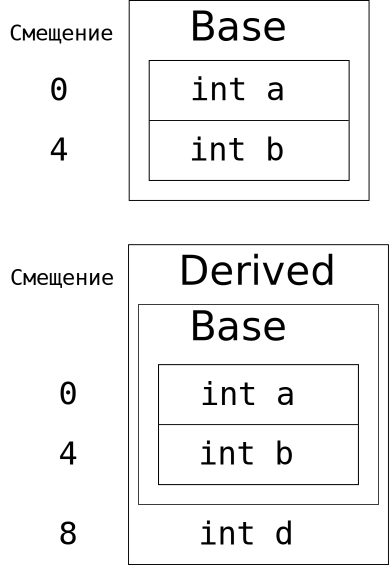
\includegraphics[width=4cm]{inheritance_layout.pdf}
  \hfill
  \caption{Расположение классов в памяти при одиночном наследовании}
  \label{inheritance_layout_fig}
\end{figure}

\paragraph{Множественное наследование}
Множественное наследование следует тем же принципам, что и одиночное. Рассмотрим код на \picref{multiple_inheritance_lst}.
\begin{figure}
\begin{lstlisting}
class Base1 {
    int a1, b1;
};

class Base2 {
    int a2, b2;
};

class Derived : public Base1, public Base2 {
    int d;
};
\end{lstlisting}
\caption{Пример множественного наследования}
\label{multiple_inheritance_lst}
\end{figure}
Расположение объектов в памяти показано на \picref{multiple_inheritance_layout_fig}.
При этом приведение указателя типа \code{Derived~*} к типу \code{Base2~*} потребует увеличения значения указателя на величину, равную размеру класса \code{Base1}, а обратное приведение --- уменьшения на ту же величину.
\begin{figure}
  \center
  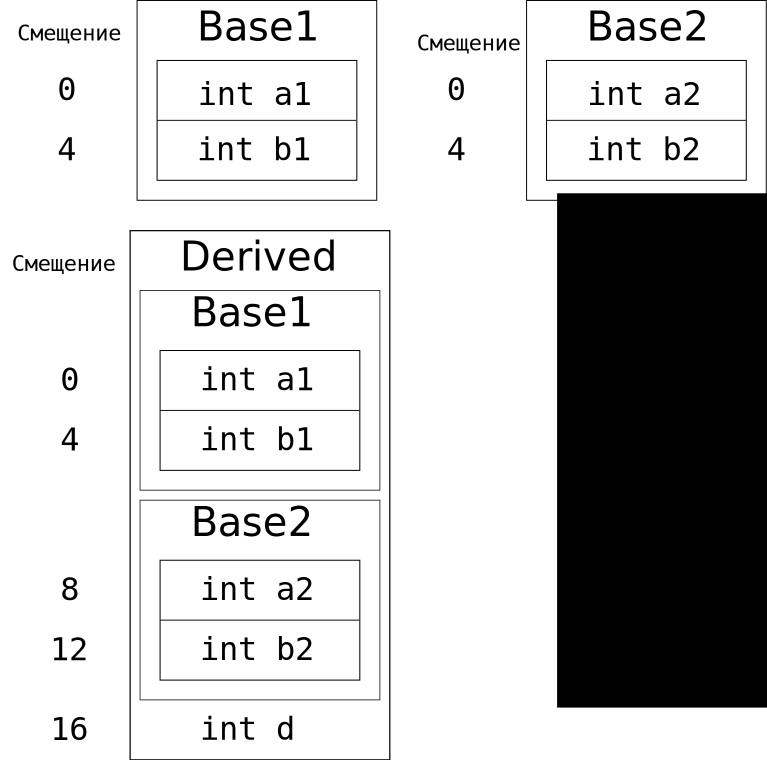
\includegraphics[width=8cm]{multiple_inheritance_layout.pdf}
  \hfill
  \caption{Расположение классов в памяти при одиночном наследовании}
  \label{multiple_inheritance_layout_fig}
\end{figure}

\subsubsection{Виртуальные функции}
\label{virtual_call}
Механизм виртуальных функций позволяет определить в базовом классе функции, которые могут быть замещены в производных классах.
При вызове такой функции через указатель на базовый класс будет вызвана функция из соответствующего производного класса.
Этот механизм реализуется при помощи \emph{таблиц виртуальных функций}.
Рассмотрим пример, показанный на \picref{virtual_functions_lst}, для компилятора g++ на 32-битной платформе.
\begin{figure}
\begin{lstlisting}
class Base {
public:
  virtual int f();
  int b;
};

class Derived {
public:
  int f();
  int d;
}
\end{lstlisting}
\caption{Пример классов с виртуальными функциями}
\label{virtual_functions_lst}
\end{figure}

В данном случае, будет создано по одной таблице виртуальных функций на каждый из классов.
Объекты каждого из классов будут иметь раскладку в памяти, показанную на \picref{memlayout_fig} (\code{vptr} --- указатель на таблицу виртуальных функций).

Сами таблицы виртуальных функций будут выглядеть так, как показано на \picref{simple_vtables_fig}.
Вызов виртуальной функции \code{f} происходит следующим образом: по указателю на \code{base} находится указатель на таблицу виртуальных функций, из таблицы берётся адрес требуемой функции, происходит вызов функции.
Например, для кода, показанного на \picref{virtual_call_lst}, компилятор g++ на 64-битной платформе сгенерирует следующий ассемблерный код.
\begin{figure}
\begin{lstlisting}
void test(Base *base) {
  base->f();
}
\end{lstlisting}
\caption{Пример вызова виртуальной функции}
\label{virtual_call_lst}
\end{figure}

\begin{minipage}[b]{\linewidth}
\vspace{0.5cm}
\begin{minipage}[t]{0.40\linewidth}
\begin{lstlisting}[language={[x86masm]Assembler}]
mov    -0x28(%rbp),%rax
mov    (%rax),%rax
mov    (%rax),%rdx
mov    -0x28(%rbp),%rax
mov    %rax,%rdi
callq  *%rdx
\end{lstlisting}
\end{minipage}
\vline
\begin{minipage}[t]{0.45\linewidth}
\begin{enumerate}
\item В регистр \code{rax} загружается адрес объекта \code{base}.
\item В регистр \code{rax} загружается значение по адресу \code{rax}. Как было показано ранее, самое первое значение в памяти занимаемой объектом является указателем на таблицу виртуальных функций.
\item В регистр \code{rdx} загружается адрес первой (со смещением $0$) функции из таблицы виртуальных функций.
\item В регистр \code{rax} загружается адрес объекта \code{base}.
\item Адрес объекта копируется в регистр \code{rdi}. Передача указателя \code{this} происходит через регистр.
\item Происходит вызов виртуальной функции.
\end{enumerate}
\end{minipage}
\vspace{0.5cm}
\end{minipage}

Этот же код выглядит во внутреннем представлении \code{Valgrind} как показано на \picref{vcall_valgrind_lst}(показан только срез, имеющий отношение к виртуальному вызову):
\begin{figure}
\begin{lstlisting}
t11 = GET:I64(40)
t10 = Add64(t11,0xFFFFFFFFFFFFFFD8:I64)
t12 = LDle:I64(t10)
t13 = LDle:I64(t12)
t14 = LDle:I64(t13)
goto {Call} t14
\end{lstlisting}
\caption{Внутреннее представление \code{Vaglrind} для вызова виртуальной функции}
\label{vcall_valgrind_lst}
\end{figure}


Заметим, что в большинстве случаев различным классам соответствуют различные таблицы виртуальных функций.
Это так потому, что класс, имеющий виртуальные функции, как правило \cite{meyers}, имеет и виртуальный деструктор, таким образом, хотя бы он будет всегда замещаться в классах-наследниках, даже если они не переопределяют других виртуальных функций.

Невозможна также ситуация, когда одному классу соответствует несколько таблиц виртуальных функций.
В том случае, если определения некоторых методов класса содержатся в заголовочном файле, и таблица виртуальных функций для данного класса будет создана и размещена в каждой из единиц трансляции, включающих этот заголовочный файл, компоновщик поместит в результирующий исполняемый файл только одну копию.

\begin{figure}
  \center
  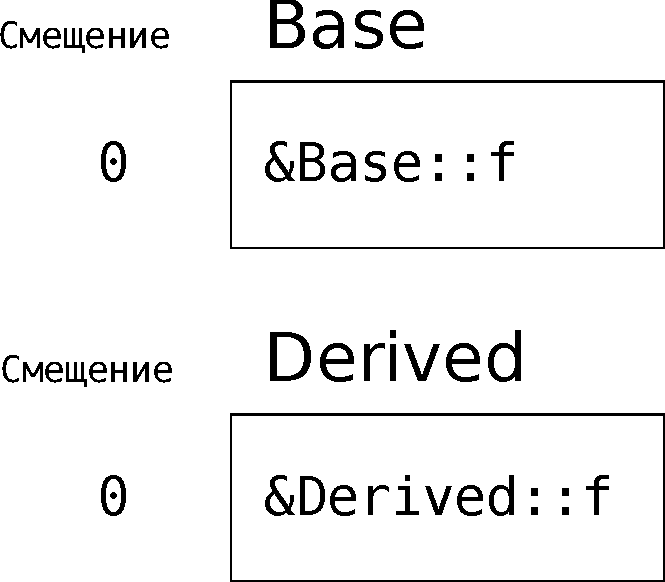
\includegraphics[width=4cm]{simple_vtables.pdf}
  \hfill
  \caption{Расположение в памяти таблиц виртуальных функций}
  \label{simple_vtables_fig}
\end{figure}

\begin{figure}
  \center
  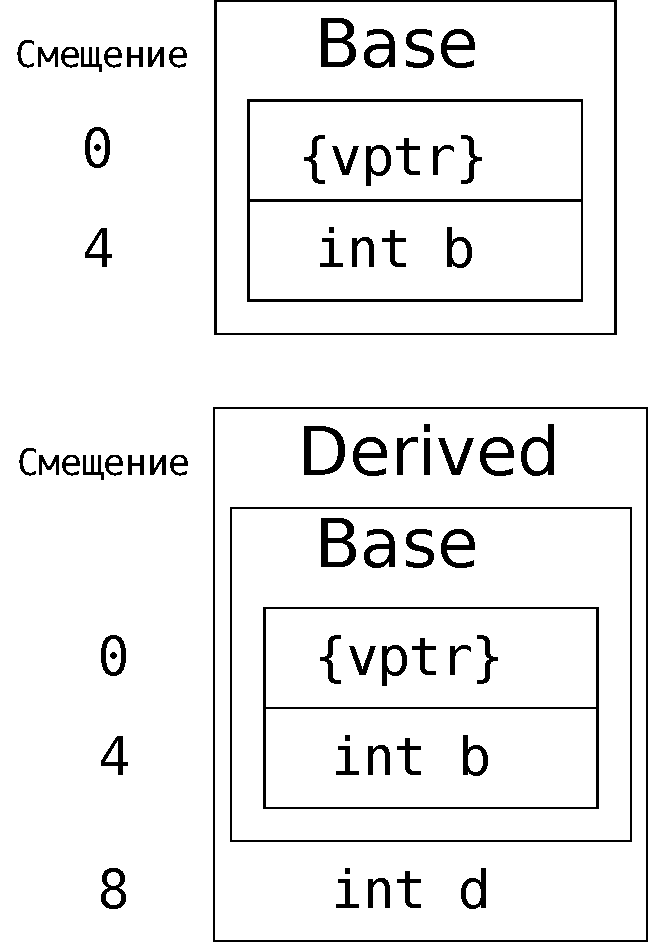
\includegraphics[width=4cm]{simple_mem_layout.pdf}
  \hfill
  \caption{Расположение классов в памяти}
  \label{memlayout_fig}
\end{figure}

\subsubsection{RTTI}
RTTI (Run-time Type Information --- информация о типах времени выполнения) представляет из себя метод получения информации о реальном типе класса по указателю на объект одного из его базовых классов.
Для хранения этой информации используются специальные структуры данных, содержащие информацию об отношении наследования классов.
Указатель на структуру, описывающую класс сохраняется в его таблице виртуальных функций\footnote{Поэтому, информация о типе времени выполнения может быть получена только для класса, имеющего виртуальные функции.}.
Как уже было показано в разделе \ref{reverse_eng_overview}, эта информация может успешно применяться для восстановления определений классов.
В данной же работе рассматривается ситуация, когда эта информация отсутствует в исполняемом файле.

\subsection{Метод решения задачи}
Исходя из вышесказанного, представляется целесообразным использовать для восстановления определений классов информацию о таблицах виртуальных функций и виртуальных вызовах, собираемую во время работы анализируемой программы.

Метод решения основывается на сборе информации о имевших место вызовах виртуальных функций в программе и последующем анализе собранной информации.
Реализованный метод позволяет восстанавливать для каждого вызова виртуальной функции получать следующие значения: адрес инструкции, осуществляющей вызов, в коде программы, адрес использованной для вызова таблицы виртуальных функций и номер вызываемой виртуальной функции в таблице.
Полученная информация накапливается во время работы анализируемой программы, сам анализ проходит после её завершения.

\subsubsection{Предварительный сбор информации}
Для выявления вызовов виртуальных функций используется метод сопоставления с образцом, описанном в разделе \ref{virtual_call}.
Также должно выполняться следующее условие: предполагаемый адрес таблицы виртуальных функций должен находиться в разделе памяти, являющимся отображением исполняемого файла и имеющего доступ только на чтение.
Каждому адресу в коде программы, который являлся вызовом виртуальной функции ставится в соответствие структура данных, называемая далее \emph{точкой вызова}.
В точке вызова сохраняется номер вызываемой виртуальной функции и множество таблиц виртуальных функций, использованных для вызова в этой точке.

Введём следующие обозначения.
Место вызова будем обозначать заглавной буквой, таблицу виртуальных функций маленькой.
Множество таблиц виртуальных функций, использованных в точке вызова будем обозначать $calles[A]$, номер вызываемой функции $fn[A]$.
\paragraph{Методы обнаружения фрагментов в машинном коде}
Существует нес\-колько методов решения этой задачи.
Основные из них --- это сигнатурный поиск и сопоставление с образцом.
При сигнатурном поиске фрагмент кода, который необходимо найти, должен быть фиксированным.
Для ускорения поиска могут быть использованы алгоритмы поиска подстроки в строке, такие как алгоритм Бойера-Мура \cite{corman}.

При сопоставлении с образцом выделяется общая структура фрагмента и формируется образец, имеющий пропуски, в которых может быть расположен произвольный код.

В данной работе используется метод сопоставления с образцом, т.к. машинный код для виртуального вызова имеет известную структуру, но конкретные значения регистров и констант могут различаться.

Как уже было описано в разделе \ref{valgrind_section}, \code{Valgrind} передаёт код анализируемой программы инструменту по блокам. Экспериментально было установлено, что вызов виртуальной функции почти всегда\footnote{Исключением является только тот случай, когда формирование блока прекращается по достижению лимита в 50 машинных инструкций. Эксперимент показывает, что описанная ситуация возникает менее, чем в 6\% случаев, что является приемлемым в нашем подходе.} попадает внутрь одного блока.
Далее, если имеет место вызов функции по статически неизвестному адресу, вычисляемому во время работы программы, формируется специальный указатель для блока, содержащий выражение, значение которого равно адресу функции, вызов которой происходит.

Введём следующую нотацию для записи сопоставляемых фрагментов.
\begin{itemize}
    \item \code{call x} --- вызов функции по адресу \code{x}.
    \item \code{x}$\leftarrow$\code{e} --- присваивание значения выражения \code{e} переменной \code{x}.
    \item \code{x}$\leftarrow$\code{[y]} --- присваивание значения, расположенного по адресу \code{y}, переменной \code{x}.
\end{itemize}
При этом будем требовать, чтобы в сопоставляемом фрагменте кода значение каждой переменной присваивалось ровно 1 раз, выражение \code{call} всегда входило в фрагмент последним.

Сопоставление участка кода и образца будем проводить с конца, используя тот факт, что в \code{Valgrind} использует \code{SSA} для внутреннего представления кода и оператор вызова функции по адресу может быть только последней инструкцией в блоке.
Сначала происходит сопоставление оператора \code{call}. Далее, сопоставление ведётся до тех пор, пока множество переменных образца, не сопоставленных с переменными блока, не пусто.

\begin{enumerate}
    \item Выбирается следующий с конца оператор \code{x}$\leftarrow$\code{y}.
    \item В блоке кода находится оператор присваивания для переменной, сопоставленной переменной образца \code{x}.
    \item Происходит сопоставление правых частей выражений. Если оно успешно, переменные образца в правой части сопоставляются соответствующим переменным блока. Если же оно не успешно, сопоставление завершается неудачей.
\end{enumerate}

Результатом сопоставления является отображение переменных образца в сопоставленные им переменные блока кода.

Для выявления виртуальных вызовов функций используются следующие два образца, показанные на \picref{vcall_pattern_0_lst} и \picref{vcall_pattern_off_lst}. Конечным результатом работы является тройка $(object,\;vtable,\;offset)$ --- адрес объекта, указатель на таблицу виртуальных функций, смещение виртуальной функции в таблице.

В случае успешного сопоставления с  образцом, показанным на \picref{vcall_pattern_0_lst}, $offset \equiv 0$.

\begin{figure}
\begin{lstlisting}
vtable <- [object]
e <- [vtable]
call e
\end{lstlisting}
\caption{Образец для сопоставления вызова виртуальной функции с индексом 0}
\label{vcall_pattern_0_lst}
\end{figure}
\begin{figure}
\begin{lstlisting}
vtable <- [object]
vtable_ref <- vtable + offset
e <- [vtable_ref]
call e
\end{lstlisting}
\caption{Образец для сопоставления вызова виртуальной функции с ненулевым индексом}
\label{vcall_pattern_off_lst}
\end{figure}

\paragraph{Методы получения информации о структуре памяти процесса}
\label{proc_map}
Одно из условий для обнаружения виртуального вызова --- возможность проверять, находится ли объект с известным адресом в области кода программы, предназначенной только для чтения.
В ОС GNU/Linux эта информация может быть считана из виртуальной файловой системы \code{proc}\footnote{Информация находится в файле \code{/proc/\{pid\}/maps}, где \code{\{pid\}} --- идентификатор процесса.}.

\subsubsection{Нахождение начала таблицы виртуальных функций}
\label{vtable_beginning_search}
В случае, когда имеет место множественное наследование, и происходит вызов виртуальной функции одного из родительских классов, будет использоваться таблица виртуальных функций, соответствующая этому родительскому классу.
Для распознавания множественного наследования необходимо найти адрес начала таблицы виртуальных функций унаследованного класса.

Рассмотрим работу метода на примере. Пусть имеется иерархия, как на \picref{vtable_start_ex_lst}.
\begin{figure}
\begin{lstlisting}
class A {
public:
    int a;
    virtual void v();
};

class B {
public:
    int b;
    virtual void w();
};

class C : public A, public B {
public:
    int c;
    void w();
};
\end{lstlisting}
\caption{Пример иерархии классов}
\label{vtable_start_ex_lst}
\end{figure}
Схема расположения объектов изображена на \picref{multiple_inheritance_scheme_fig}.
Можно видеть, что функция \code{C::w} была помещена в продолжении таблицы виртуальных функций класса \code{A}, а для класса \code{B} была создана отдельная таблица виртуальных функций.
Также, начало объекта класса \code{B} не совпадает с началом объекта класса \code{C}.
Поэтому в случае вызова метода класса \code{B} у объекта типа \code{C} требуется модифицировать указатель \code{this}.
Для этого существует специальная функция (\code{thunk}), добавляющая смещение к параметру \code{this} и передающая управление соответствующему методу класса \code{B}.

Реализованный алгоритм восстановления определений классов требует для своей работы метод для получения указателя на таблицу виртуальных функций того объекта, для которого происходит вызов виртуальной функции.
В случае с вызовом метода класса \code{B}, этот указатель (нижняя стрелка на \picref{multiple_inheritance_scheme_fig}) не будет совпадать с реальным (верхняя стрелка на \picref{multiple_inheritance_scheme_fig}).

Здесь \code{top\_offset} является элементом внутренней разметки таблицы виртуальных функций.
\code{vptr} --- указатель на таблицу виртуальных функций, \code{typeinfo} --- указатель на структуру данных \code{RTTI}, либо $0$, если приложение скомпилировано с отключённым \code{RTTI}.
Поле \code{top\_offset} всегда заполняется таким образом, что оно равно нулю только для таблицы виртуальных функций наиболее точного типа.

Метод нахождения начала таблицы виртуальных функций получает на вход адрес таблицы виртуальных функций, возможно, принадлежащий одному из подклассов объекта, для которого происходит виртуальный вызов.
Результатом работы является указатель на начало таблицы виртуальных функций объекта, для которого происходит виртуальный вызов.
Выходное значение может совпадать со входным, например, если в данном случае нет множественного наследования.

Алгоритм представлен на \picref{find_vtable_begin_lst}.
\begin{figure}
\begin{lstlisting}
findVtableBeginning(address) {
    typeinfo = address[-1]
    top_offset = address[-2]
    while top_offset != 0 {
        repeat
            --address
        until address[-1] != typeinfo
        top_offset = address[-2]
    }
    return address
}
\end{lstlisting}
\caption{Псевдокод алгоритма для нахождения начала таблицы виртуальных функций}
\label{find_vtable_begin_lst}
\end{figure}

В строках 1--2 происходит начальная инициализация полей.
В цикле \code{while} происходит поиск таблицы виртуальных функций с \code{top\_offset}, равным 0.
Если текущая таблица виртуальных функций не удовлетворяет этому требованию, то находится предыдущая таблица с таким же значением \code{typeinfo}.

Алгоритм опирается на тот факт, что значение \code{typeinfo} однозначно определяет наличие следующей таблицы виртуальных функций.
Это выполняется даже в том случае, когда указатель \code{typeinfo} равен 0, т.к. никаких других полей с нулевым значением в таблице виртуальных функций быть не может.

\begin{figure}
  \center
  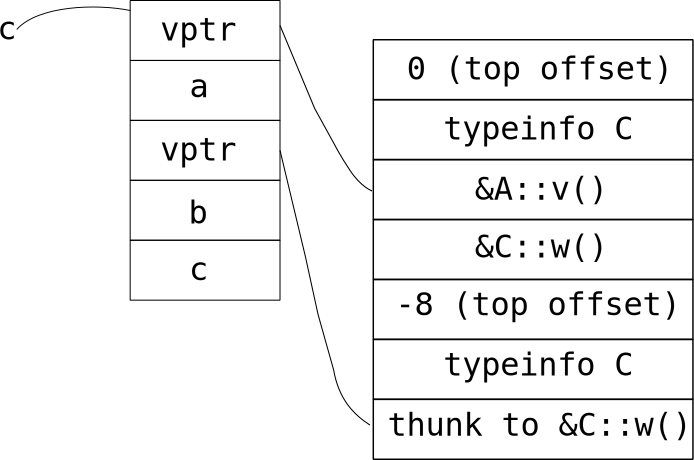
\includegraphics[width=8cm]{multiple_inheritance_scheme.pdf}
  \hfill
  \caption{Схема таблицы виртуальных функций в случае множественного наследования.}
  \label{multiple_inheritance_scheme_fig}
\end{figure}

\subsubsection{Нахождение размера таблицы виртуальных функций}
Для каждой из найденных таблиц виртуальных функций также является важным определить количество адресов начала виртуальных функций, содержащихся в ней.
Реализованный алгоритм последовательно просматривает таблицу до тех пор, пока встречаемые указатели могут представлять собой указатели на функции.
Проверка этого свойства заключается в проверке того, что значением указателя является адрес, расположенный в области памяти только для чтения.
Псевдокод алгоритма представлен на \picref{find_vtable_size_lst}.
\begin{figure}
\begin{lstlisting}
getVtableSize(address) {
    i = 0
    while address[i] is in readonly section {
        ++i
    }
    return i
}
\end{lstlisting}
\caption{Псевдокод алгоритма для нахождения размера таблицы виртуальных функций}
\label{find_vtable_size_lst}
\end{figure}

\subsubsection{Построение иерархии мест вызовов}
Предварительно заметим, что каждому из мест вызова в исходном коде анализируемой программы соответствует оператор вызова метода объекта.
При этом, объект имеет тип, известный во время компиляции, но не известный во время работы программы.
Идея следующего алгоритма состоит в первоначальном назначении каждому месту вызова уникального типа.
Далее, используя собранную информацию, типы, связанные с местами вызова, будут объединяться.
В ходе описания работы алгоритма отождествляются понятия места вызова и типа, ему соответствующего.
Таким образом, объединение двух мест вызова будет означать, что им соответствуют одинаковые типы.

Конечной целью работы алгоритма является некоторая иерархия типов, не противоречащая собранной информации.
Другими словами, если бы в исходной программе в местах вызова объекты бы имели типы, полученные в результате работы алгоритма,
то компилятор мог бы сгенерировать таблицы виртуальных функций, полученные в результате анализа программы, и, кроме того, все вызовы виртуальных функций,
сделанные анализируемой программой были бы возможны.

На типы, соответствующие местам вызова накладываются важные условия.
\begin{itemize}
\item Тип может иметь только один базовый тип. Восстановление множественного наследования происходит в конце работы алгоритма;
\item Считаем, что в типе (классе), соответствующему месту вызова $A$ определено ровно $fn[A]$ виртуальных функций.
\end{itemize}
Второй пункт можно проиллюстрировать следующим отрывком кода, показанным на \picref{min_vsize_ex_lst}.
\begin{figure}
\begin{lstlisting}
class Base {
public:
    virtual void f();
};

class Derived : public Base {
    void f();
    virtual void g();
};

void fun(Derived *d) {
    d->f();
    static_cast<Base *>(d)->f();
}
\end{lstlisting}
\caption{Пример вызова виртуальной функции через указатель на базовый класс}
\label{min_vsize_ex_lst}
\end{figure}

Здесь, выражения в строках \code{12} и \code{13} абсолютно идентичны в смысле семантики, определяемой языком и кода, генерируемого компилятором.
Следовательно, проведя анализ программы, можно достоверно утверждать только что имеет место вызов, показанный в строке \code{13}.

Алгоритм состоит из пяти фаз.
Все фазы описаны в виде некоторого условия и соответствующего преобразования отношения наследования, либо множества мест вызова.
Каждая из фаз выполняется до тех пор, пока выполняется определённое в ней условие.

\paragraph{Продвижение множеств использованных таблиц виртуальных функций}
Пусть есть два места вызова $A$ и $B$, в которых происходил вывоз методов одного класса и $fn[A] \geq fn[B]$.
Тогда легко видеть, что тип $A$ должен быть наследником $B$, возможно неявным; будем обозначать этот факт как $A \rightsquigarrow B$.
Из этого можно заключить, что все вызовы методов объектов, сделанные через $B$, могут также быть сделаны и через $A$.

Выразим это более формально:
\begin{eqnarray*}
\forall A,\;B:\qquad callees[A] \cap callees[B] \neq \varnothing \wedge fn[A] \geq fn[B]\\
\implies callees[A] := callees[A] \cup callees[B]
\end{eqnarray*}

\paragraph{Слияние мест вызовов}
Если существуют два места вызова $A$ и $B$, такие что $fn[A] = fn[B]$ и $A \rightsquigarrow B$, то типы $A$ и $B$ совпадают.
Это верно в силу требования, которое мы предъявляем к классам, соответствующим точкам вызова: при наследовании количество функций в классе должно строго увеличиваться.

Формально:
\begin{eqnarray*}
\forall A,\;B\qquad fn[A] = fn[B] \wedge callees[A] \cap callees[B] \neq \varnothing\\
\implies A := B
\end{eqnarray*}

\paragraph{Сортировка мест вызовов}
Первая фаза алгоритма уже даёт некоторое отношение наследования для классов: известно, какие классы должны наследоваться от каких, но на первой фазе не было ясно, какое наследование должно быть прямым, а какое неявным. Данная фаза алгоритма позволяет построить явное отношение наследования.

Фиксируем класс $A$ и рассмотрим множество \[\mathcal{P} = \{B:\; A \rightsquigarrow B\}\]
Если $\mathcal{P} = \varnothing$, то мы можем заключить, что класс $A$ не является наследником каких-либо классов. Если же $\mathcal{P}$ не пусто, то рассмотрим класс \[P = \arg \min_{P \in \mathcal{P}}fn[P]\]

Стоит отметить, что $P$ определяется единственным образом, т.к. \[\forall B_1,\;B_2 \in \mathcal{P}\; B_1 \neq B_2 \implies fn[B_1] \neq fn[B_2],\]
это свойство было установлено на второй фазе алгоритма.
Положим что $A$ является прямым наследником $P$, т.е. $A \rightarrow P$.

Легко видеть, что отношение наследования ``$\rightarrow$'' не противоречит отношению неявного наследования ``$\rightsquigarrow$''.

Формально:
\begin{eqnarray*}
\forall A\qquad A \rightarrow \begin{cases}
\varnothing,\; \overline{\exists} B:\; A \rightsquigarrow B,\\
\arg\min\limits_{B:\; A \rightsquigarrow B}fn[B]
\end{cases}
\end{eqnarray*}

\paragraph{Сокращение цепочек}
Каждое место вызова, которое наследуется только 1 раз может быть объединено с местом вызова, родителем которого оно является.
Данная фаза позволяет избавиться от цепочек мест вызова, возникающих при вызове нескольких методов одного класса.

Формально:
\begin{eqnarray*}
\forall A,\;B:\qquad A \rightarrow B\;\wedge\;|\{C:\; C \rightarrow B\}| = 1\\
\implies B := A
\end{eqnarray*}

\paragraph{Восстановление множественного наследования}
После работы предыдущих фаз алгоритма, для каждой из таблиц виртуальных функций находится родительская таблица виртуальных функций в соответствии с алгоритмом, описанным в главе \ref{vtable_beginning_search}.
После этого, в имеющейся иерархии таблицы виртуальных функций, являющиеся частями других таблиц виртуальных функций, заменяются на их родительские таблицы виртуальных функций.

\newpage
\section{Реализация}
Описанный в работе инструмент реализован на языке Си++ в рамках среды \code{Valgrind}. Объём исходного кода инструмента --- около 1500 строк.
Инструмент работает на 32- и 64-разрядных архитектурах под управлением ОС \code{GNU/Linux}.
Реализованный инструмент состоит из двух подсистем:
\begin{itemize}
    \item Подсистема сбора информации о виртуальных вызовах;
    \item Подсистема восстановления иерархии классов.
\end{itemize}
Такая организация позволит при необходимости легко перейти к другому методу сбора информации о виртуальных вызовах, например, на основе срезов трасс работы программы.

Поддерживается два варианта для вывода результата анализа: описание графа наследования на языке \code{dot}, которое может быть визуализировано с помощью пакета \code{Graphviz}, и определения классов на языке Си++.
Стоит отметить, что никакой информации о содержимом классов не восстанавливается, поэтому тела сгенерированных классов всегда пусты.

Общая схема таботы инструмента выглядит следующим образом:
\begin{enumerate}
    \item \code{Valgrind} загружает исполняемую программу в память и вызывает фукнцию инициализации инструмента.
    \item Инструмент считывает карту отображаемой памяти для анализируемой программы.
    \item Для каждого из базовых блоков программы \code{Valgrind} вызывает специальную функцию инстумента, которая может модифицировать исполняемый код модифицируемой программы. Инструмет перед каждым из обнаруженных вызовов виртуальных функций вставляет вызов функции-перехватчика, позволяющей сохранить адрес объекта, вызов виртуального метода которого происходит, адрес его таблицы виртуальных функций и номер вызываемой функции в этой таблице.
    \item Модифицированный код анализируемой программы выполняется, при этом выполняется сбор указанной информации о вызовах виртуальных функций.
    \item Анализируемая программа завершается, \code{Valgrind} вызвает функцию завершения работы инструмента.
    \item Инструмент анализирует собранную информацию о вызовах виртуальных функций и восстанавливает отношение наследования для классов анализируемой программы.
    \item Инструмент выводит отношение наследования в формате, определяемом флагом командной строки, на стандартный поток вывода.
\end{enumerate}

\subsection{Формат описания отображений памяти для процесса в ОС \code{Linux}}
Данный раздел содержит описание формата, используемого в ОС \code{Linux} для описания отображённой памяти процесса.
Информация содержится в файле \code{/proc/\{pid\}/maps}, где \code{\{pid\}} --- идентификатор процесса.

Файл состоит строк, каждая из которых описывает одно отображение.
В качестве примера часть такого файла для командной оболочки \code{zsh}, работяющей на платформе \code{x86\_64} показана на \picref{zsh_maps_lst}.

\begin{figure}[h]
\begin{lstlisting}[basicstyle=\tiny]
00400000-00491000 r-xp 00000000 fd:00 483439              /bin/zsh
00690000-00691000 r--p 00090000 fd:00 483439              /bin/zsh
00691000-00697000 rw-p 00091000 fd:00 483439              /bin/zsh
00697000-006aa000 rw-p 00000000 00:00 0
020fc000-02201000 rw-p 00000000 00:00 0                   [heap]
7fea9104c000-7fea91053000 r-xp 00000000 fd:00 486810      /usr/lib64/zsh/4.3.10/zsh/zutil.so
7fea91053000-7fea91252000 ---p 00007000 fd:00 486810      /usr/lib64/zsh/4.3.10/zsh/zutil.so
7fea91252000-7fea91253000 r--p 00006000 fd:00 486810      /usr/lib64/zsh/4.3.10/zsh/zutil.so
7fea91253000-7fea91254000 rw-p 00007000 fd:00 486810      /usr/lib64/zsh/4.3.10/zsh/zutil.so
7fea91254000-7fea91277000 r-xp 00000000 fd:00 486821      /usr/lib64/zsh/4.3.10/zsh/complete.so
7fea91277000-7fea91477000 ---p 00023000 fd:00 486821      /usr/lib64/zsh/4.3.10/zsh/complete.so
7fea91477000-7fea91478000 r--p 00023000 fd:00 486821      /usr/lib64/zsh/4.3.10/zsh/complete.so
7fea91478000-7fea91479000 rw-p 00024000 fd:00 486821      /usr/lib64/zsh/4.3.10/zsh/complete.so
\end{lstlisting}
\caption{Пример части файла \code{/proc/\{pid\}/maps} для командной оболочки \code{zsh}}
\label{zsh_maps_lst}
\end{figure}

Каждая из строк содержит следующие поля:
\begin{enumerate}
    \item Диапазон адресов. Например: \code{08048000-08056000}
    \item Права доступа. Например: \code{r-xp}
    \item Смещение в файле. Например: \code{r-xp}
    \item Адрес устройства. Например: \code{03:0c}
    \item Номер индексного дескриптора. Например: \code{64593}
    \item Имя отображённого файла. Например: \code{/bin/zsh}
\end{enumerate}

В нашем случае, интерес представляют только первое и второе поля.
Права доступа задаются набором следующих флагов:
\begin{itemize}
    \item \code{r} --- Право на чтение.
    \item \code{w} --- Право на запись.
    \item \code{x} --- Право на исполнение. Т.е. в этом участке памяти может размещаться исполняемый код.
    \item \code{s} --- Область памяти разделяется с другим процессом.
    \item \code{p} --- Область памяти разделяется с другим процессом и используется копирование при записи (англ. Copy on Write).
\end{itemize}

\subsection{Поддержка Си++}
Сама среда \code{Valgrind} реализована на языке Си. Инструменты, реализованные с помощью этой среды также должны быть реализованы на этом языке.
Размещение в одном адресном пространстве с анализируемой программой накладывает важное ограничение: ни ядро \code{Valgrind}, ни инструмент не могут использовать стандартные библиотеки.
Причина для введения этого ограничения заключается в том, что может возникнуть ситуация, когда одна и та же функция будет исполняться анализируемой программой и самим \code{Valgrind}'ом.
Поэтому для использования \code{STL}, требуемые части реализации статически связываются с ядром \code{Valgrind}.
Реализация вспомогательных функций механизмов исключений и динамической информации о типах находится в разделяемой библиотеке, поэтому единственной способ избавиться от этой зависимости --- это отказаться от использования этих механизмов.

В связи с этим используется модифицированное подмножество библиотеки \code{STL}, в котором исключено использование операторов \code{dynamic\_cast}, \code{typeid}, \code{throw}. Таким образом, отсутствует возможность обработки ошибочных ситуаций, и при их возникновении вызывается функция аварийного завершения.

При заявленных ограничениях в инструменте успешно были использованы следующие компоненты \code{STL}.
\begin{itemize}
    \item \code{algorithm}
    \item \code{map}
    \item \code{set}
    \item \code{string}
    \item \code{vector}
    \item \code{tr1/unordered\_map}
    \item \code{tr1/unordered\_set}
\end{itemize}
При этом потеребовалась модификация лишь одного из файлов библиотеки, \code{tr1/functional}, который включается в перечисленные выше файлы.

\newpage
\section{Экспериментальные результаты}
В этом разделе будут представлены результаты работы инструмента на некоторых программах. Во всех примерах, кроме последнего, используется формат вывода в виде кода на языке Си++.

\subsection{Одиночное наследование}
Командная строка для запуска:
\[\mbox{\code{\$ valgrind -{}-tool=tdheap2 -{}-output=cpp ./single-inheritance}}\]
Исходная программа и результат работы инструмента показаны на \picref{single_inheritance_ex_lst}.
Как можно видеть, восстановленная иерархия соответствует исходной.
При этом выделен базовый класс, содержащий одну виртуальную функцию, от которого унаследованы два восстановленных класса.

\begin{figure}[h!]
\begin{minipage}[t]{0.45\linewidth}
\caption*{Исходная программа}
\begin{lstlisting}
struct A {
    virtual void f() {}
};

struct B : A {
    void f() {}
};

void f(A *a) {
    a->f();
}

int main() {
    A a;
    B b;
    f(&a);
    f(&b);

    return 0;
}
\end{lstlisting}
\end{minipage}
\begin{minipage}[t]{0.5\linewidth}
\caption*{Результат работы инструмента}
\begin{lstlisting}
class x4006E1 {
//Interface
// 0x4006E1@./single-inheritance
// Functions count: 1
// Times inherited: 2
};
class x4008D0 : public x4006E1 {
// 0x4008D0@./single-inheritance
// Functions count 1
// Class name: 1A
};
class x4008B0 : public x4006E1 {
// 0x4008B0@./single-inheritance
// Functions count 1
// Class name: 1B
};
\end{lstlisting}
\end{minipage}
\caption{Пример кода с одиночным наследованием}
\label{single_inheritance_ex_lst}
\end{figure}

\subsection{Наследование от одного базового класса}
Командная строка для запуска:
\[\mbox{\code{\$ valgrind -{}-tool=tdheap2 -{}-output=cpp ./chain-inheritance}}\]
Исходная программа и результат работы инструмента показаны на \picref{chain_inheritance_ex_lst}.
Также, как и в предыдущем случае, выделен общий базовый класс, наследниками которого являются все восстановленные классы.

\begin{figure}[h!]
\begin{minipage}[t]{0.45\linewidth}
\caption*{Исходная программа}
\begin{lstlisting}
struct A {
    virtual void f() {}
};

struct B : A  {
    void f() {}
};

struct C :  B {
    void f() {}
};


void f(A *a) {
    a->f();
}

int main() {
    A a;
    B b;
    C c;
    f(&a);
    f(&b);
    f(&c);

    return 0;
}
\end{lstlisting}
\end{minipage}
\begin{minipage}[t]{0.5\linewidth}
\caption*{Результат работы инструмента}
\begin{lstlisting}
class x4006E1 {
//Interface
// 0x4006E1@./chain-inheritance
// Functions count: 1
// Times inherited: 3
};
class x400950 : public x4006E1 {
// 0x400950@./chain-inheritance
// Functions count 1
// Class name: 1A
};
class x400930 : public x4006E1 {
// 0x400930@./chain-inheritance
// Functions count 1
// Class name: 1B
};
class x400910 : public x4006E1 {
// 0x400910@./chain-inheritance
// Functions count 1
// Class name: 1C
};
\end{lstlisting}
\end{minipage}
\caption{Пример кода с наследованием от одного базового класса}
\label{chain_inheritance_ex_lst}
\end{figure}

\subsection{Множественное наследование}
Командная строка для запуска:
\[\mbox{\code{\$ valgrind -{}-tool=tdheap2 -{}-output=cpp ./multiple-inheritance}}\]
Исходная программа и результат работы инструмента показаны на \picref{multiple_inheritance_ex_lst}.
Выделены два базовых класса, наследниками которых являются унаследованные классы.

\begin{figure}[h!]
\begin{minipage}[t]{0.45\linewidth}
\caption*{Исходная программа}
\begin{lstlisting}
struct A {
    virtual void f() {}
};

struct B  {
    virtual void g() {}
};

struct C : A, B {
    void f() {}
    void g() {}
};


void f(A *a) {
    a->f();
}

void g(B *b) {
    b->g();
}

int main() {
    A a;
    B b;
    C c;
    f(&a);
    f(&c);
    g(&b);
    g(&c);

    return 0;
}
\end{lstlisting}
\end{minipage}
\begin{minipage}[t]{0.55\linewidth}
\caption*{Результат работы инструмента}
\begin{lstlisting}
class x400702 {
//Interface
// 0x400702@./multiple-inheritance
// Functions count: 1
// Times inherited: 2
};
class x4006E1 {
//Interface
// 0x4006E1@./multiple-inheritance
// Functions count: 1
// Times inherited: 2
};
class x400970 :
    public x400702, x4006E1 {
// 0x400970@./multiple-inheritance
// Functions count 2
// Class name: 1C
};
class x4009D0 : public x4006E1 {
// 0x4009D0@./multiple-inheritance
// Functions count 1
// Class name: 1A
};
class x4009B0 : public x400702 {
// 0x4009B0@./multiple-inheritance
// Functions count 1
// Class name: 1B
};
\end{lstlisting}
\end{minipage}
\caption{Пример кода со множественным наследованием}
\label{multiple_inheritance_ex_lst}
\end{figure}

\subsection{Реальная программа}
Командная строка для запуска:
\[\mbox{\code{\$ valgrind -{}-tool=tdheap2 -{}-output=dot /usr/bin/rekonq}}\]
Результат работы инструмента при запуске его на браузере \code{rekonq} \cite{rekonq} показан на \picref{rekonq_res_fig} (показана только одна из компонент связности полученного графа).
В данном случае, из-за размера получаемой иерархии классов, представлен не код на языке Си++, а графическое выражение отношения наследования, полученное с помощью пакета программ \code{Graphviz}.

\begin{figure}[b]
  \center
  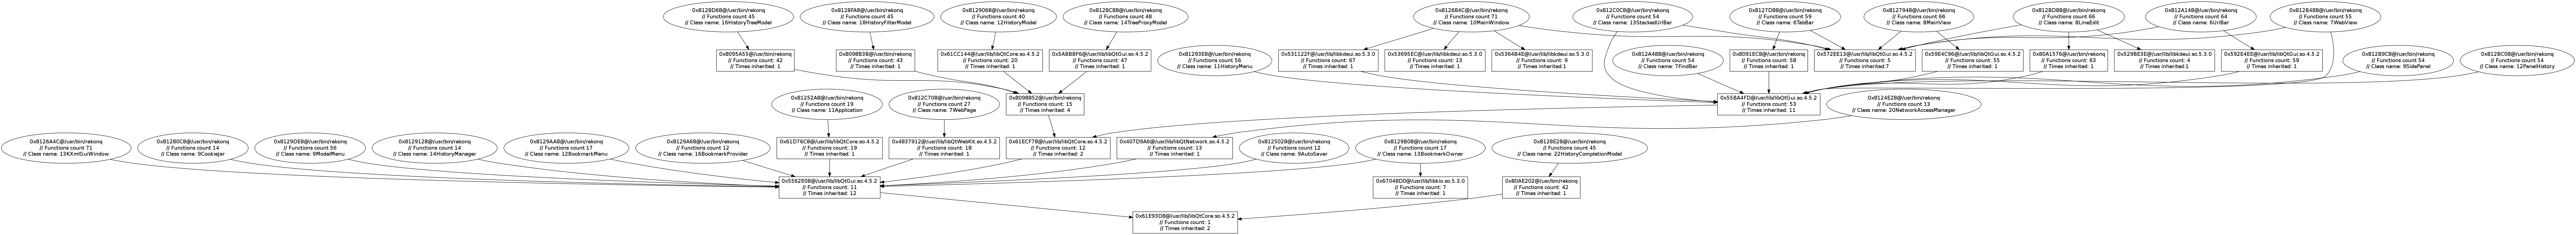
\includegraphics[width=\textwidth]{rekonq-hier.png}
  \hfill
  \caption{Результат работы инструмента на браузере \code{rekonq}}
  \label{rekonq_res_fig}
\end{figure}

\clearpage
\newpage
%\addcontentsline{toc}{section}{Заключение}
\section{Заключение}
В данной работе показана значимость подзадачи восстановления полиморфных иерархий классов в задаче обратной инженерии.
Продемонстрировано применение динамического анализа бинарного кода к задаче восстановления полиморфных иерархий.
Реализованный метод решения задачи использует метод сопоставления с образцом для динамического выделения вызовов виртуальных функций в бинарном коде.
В последствии, иерархия классов восстанавливается с помощью анализа множеств таблиц виртуальных функций, использованных в каждом из мест вызовов виртуальных функций.
Даётся описание реализованного инструмента для решения данной задачи.

Полученные результаты позволяют говорить о целесообразности применения метода динамического анализа к решаемой задаче.
Применение такого метода, при соответствующем подборе входных данных для анализируемой программы, обеспечивающим покрытие интересующих исследователя участков кода, позволяет получать иерархию классов, которая <<объясняет>> сделанные виртуальные вызовы.
Другими словами, такую иерархию, в которой все сделанные вызовы виртуальных функций были бы возможны, и таблицы виртуальных функций имели бы такой-же вид, как и в анализируемой программе.

%% Надо вывести все рисунки до списка литературы
\clearpage

\newpage
\addcontentsline{toc}{section}{Литература}
\begin{thebibliography}{9}

    \bibitem{valgrind} Nicholas Nethercote. Julian Seward. Valgrind: A Framework for Heavyweight Dynamic Binary Instrumentation. Proceedings of ACM SIGPLAN 2007 Conference on Programming Language Design and Implementation (PLDI 2007), San Diego, California, USA, June 2007.

    \bibitem{abstracttypes} Philip J. Guo. Jeff H. Perkins. Stephen McCamant. Michael D. Ernst. Dynamic Inference of Abstract Types. Proceedings of the International Symposium on Software Testing and Analysis, Portland, Maine, USA, 2006.

    \bibitem{typechecking} Michael Burrows. Stephen N. Freund. Janet L. Wiener. Run-Time Type Checking for Binary Programs. International Conference on Compiler Construction, Warsaw, Poland, April 2003.

    \bibitem{strstr} Бьерн Страуструп. Язык программирования С++. М.: Бином, 2006. 1100 с.
    \bibitem{reversing_cpp}P. Sabanal, M. Yason. Reversing C++. Black Hat DC, Arlington, Virginia, USA, 2007.
    \bibitem{real_decomp} M. Van Emmerik, T. Waddington. Using a decompiler for real-world source recovery. Proceedings of 11th Working Conference on Reverse Engineering, с. 27-36. 2004.
    \bibitem{boomerang} Mike Van Emmerik, Gerard Krol, Trent Waddington. A general, open source, retargetable decompiler of machine code programs. [HTML] (\code{http://boomerang.sourceforge.net})
    \bibitem{ida_pro} Ilfak Guilfanov. The IDA Pro Disassembler and Debugger. [HTML] (\code{http://www.hex-rays.com/idapro/})
    \bibitem{rekonq} rekonq WebKit KDE browser. [HTML] (\code{http://rekonq.sourceforge.net/})
    \bibitem{corman} Т.~Кормен, Ч.~Лейзерсон, Р.~Ривест. Алгоритмы: построение и анализ. М.: МЦНМО, 2002. 960 с.
    \bibitem{meyers} Scott Meyers. Effective C++: 55 Specific Ways to Improve Your Programs and Designs. ISBN 0-321-33487-6, 1992.
    \bibitem{aho_compilers} Альфред В. Ахо, Моника С. Лам, Рави Сети, Джеффри Д. Ульман. Компиляторы: принципы, технологии и инструментарий. — 2-е изд. — М.: Вильямс, 2008
    \bibitem{cpp_standard} ANSI ISO/IEC FDIS 14882 standard: Programming languages --- C++.
\end{thebibliography}


\end{document}

%rtti
%ооп
%vtable
%this
%abi
%отношение ассоциации (uml)
%поток данных
%поток управления
%алиас
%статический анализ
%динамический анализ
